\documentclass[tikz]{standalone}
\usepackage{tikz}
\usetikzlibrary{positioning, graphs}
\usetikzlibrary{graphs.standard}
\begin{document}
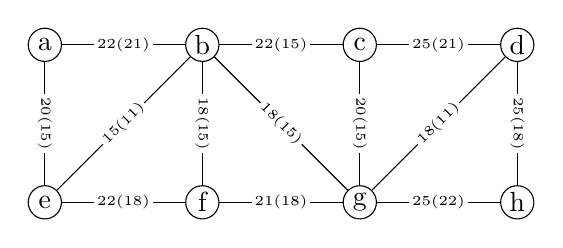
\begin{tikzpicture}
\begin{scope}
		[vertex/.style={draw,circle,inner sep = 0em, minimum size = 1.2em},
		 edgelabel/.style = {fill = white, inner sep = 0.1em, font=\tiny, sloped}]
		\node[vertex] (a) at (0,0) {a};
		\node[vertex] (b) at (2,0) {b};
		\node[vertex] (c) at (4,0) {c};
		\node[vertex] (d) at (6,0) {d};
		\node[vertex] (e) at (0,-2) {e};
		\node[vertex] (f) at (2,-2) {f};
		\node[vertex] (g) at (4,-2) {g};
		\node[vertex] (h) at (6,-2) {h};
		
		\draw[-] (a) to node[edgelabel]{$22(21)$} (b);
		\draw[-] (a) to node[edgelabel]{$20(15)$} (e);
		\draw[-] (b) to node[edgelabel]{$15(11)$} (e);
		\draw[-] (b) to node[edgelabel]{$18(15)$} (f);
		\draw[-] (b) to node[edgelabel]{$18(15)$} (g);
		\draw[-] (b) to node[edgelabel]{$22(15)$} (c);
		\draw[-] (c) to node[edgelabel]{$20(15)$} (g);
		\draw[-] (c) to node[edgelabel]{$25(21)$} (d);
		\draw[-] (d) to node[edgelabel]{$18(11)$} (g);
		\draw[-] (d) to node[edgelabel]{$25(18)$} (h);
		\draw[-] (e) to node[edgelabel]{$22(18)$} (f);
		\draw[-] (f) to node[edgelabel]{$21(18)$} (g);
		\draw[-] (g) to node[edgelabel]{$25(22)$} (h);
\end{scope}
\end{tikzpicture}
\end{document}